\documentclass[tikz,border=10pt]{standalone}
% Scale s = 0.015385 cm per pixel (longest ink side = 8 cm)
\begin{document}
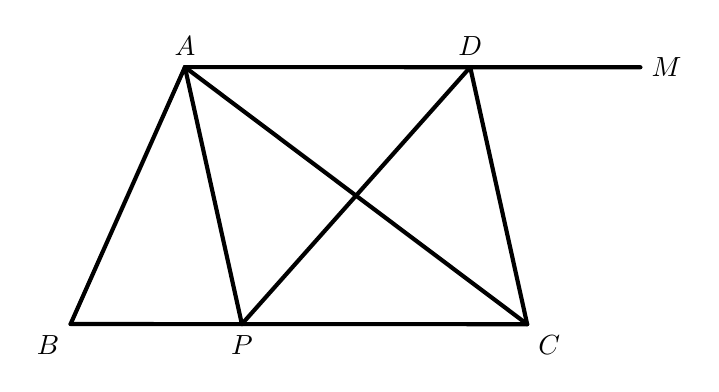
\begin{tikzpicture}[line width=1.5pt, line join=round, line cap=round]
  % Named points (coordinates unchanged from v1)
  \coordinate (B) at (-3.514136328519992,-1.6241538962894766);
  \coordinate (P) at (-1.338673596091072,-1.6248440581611268);
  \coordinate (C) at (2.2848051545271466,-1.6259936006649502);
  \coordinate (A) at (-2.062176407975804,1.638992132202937);
  \coordinate (D) at (1.5613023426424149,1.6378425896991138);
  \coordinate (M) at (3.7228788354173066,1.6371568332135025);

  % Bottom line B--C (through P)
  \draw (B) -- (C);
  % Top line A--M (through D)
  \draw (A) -- (M);
  % Remaining segments
  \draw (B) -- (A);
  \draw (A) -- (P);
  \draw (A) -- (C);
  \draw (P) -- (D);
  \draw (D) -- (C);

  % Labels, placed after all draw commands
  \node[above] at (A) {$A$};
  \node[above] at (D) {$D$};
  \node[right] at (M) {$M$};
  \node[below left] at (B) {$B$};
  \node[below] at (P) {$P$};
  \node[below right] at (C) {$C$};
\end{tikzpicture}
\end{document}
% GEOAGENT_REPAIR_V1 c18a466396f54661 feb06c8e623b1a70948e2c42016114f8233b2d1621b48c5b7bb7a099cc49e25b
